\chapter{Related work}
\label{cha:related}

This section focuses on the work of other researchers who approached the problem of automated road network generation. A quite comprehensive approach was published by Yoav I.\ H.\ Parish and Pascal Mueller in their paper \emph{"Procedural Modeling of Cities"} in $2001$. They present a system called \emph{CityEngine} which is capable of modeling a complete city using just a small set of both geographical and statistical input data. The input data, including elevation maps, water maps, population density or height maps e.g., is used by the system in order to create both the cities traffic network as well as the buildings. As this work also focuses on the generation of road networks, only the corresponding parts of the \emph{CityEngine} are described hereinafter briefly.\\

\noindent
For the generation of the cities road network Parish and Mueller introduced a L-System that acts upon two rule sets, namely \emph{global goals} and \emph{local constraints}. In \cite{parish01} the chosen road pattern and the population density information extracted from the input data are designated to belong to the global goals. Those goals are primarily considered to define initial values for the L-System's productions, a refinement of those values is done by the appliance of the local contraints function. This function basically executes the following steps:\\

\begin{itemize}
	\item Check whether the recently inserted road segment ends inside or crosses an illegal area, e.g.\ water.
	\item Check whether the inserted road segment intersects an already existing segment.
	\item Search for other road segments and crossings which are within a specified distance to the segments end.\\
\end{itemize}

\noindent
Subsequently the L-System is capable of adapting itself so it fits both the global goals and the local constraints. Segments in illegal areas for example are rotated or pruned until they do not exceed the legal limits any more. What's more, if the system identifies that the road segment is close to intersection, the segment is extended in such a way that an intersection with an existing segment is formed. The same applies to crossings respectively. Figure \ref{fig:localconstraints} gives an impression of possible local contraints, showing the adoptions the L-System makes according to the underyling rule sets. The proposed parameters correspond to the ones proposed by the global goals, the modified parameters depict the changes which have been applied taking the local contraints into consideration.\\

\begin{figure}[H]
\begin{center}
\includegraphics[width=0.72\linewidth]{images/localconstraints}
\end{center}
\caption{Examples for local constraints \cite{parish01}}
\label{fig:localconstraints}
\end{figure}

\noindent
Because of the fact the L-System adopts itself in order to fit it's own requirements Parish and Mueller entitle their system as a \emph{self-sensitive L-System}. Before rendering the generated street network a smoothing method is applied to all roads with high curvature in order to make them look more realistic. Figure \ref{fig:manhattan} illustrates a road system for the city of Manhattan which was created using the \emph{CityEngine} (left) compared to a real road map of Manhattan (right).\\

\begin{figure}[H]
\begin{center}
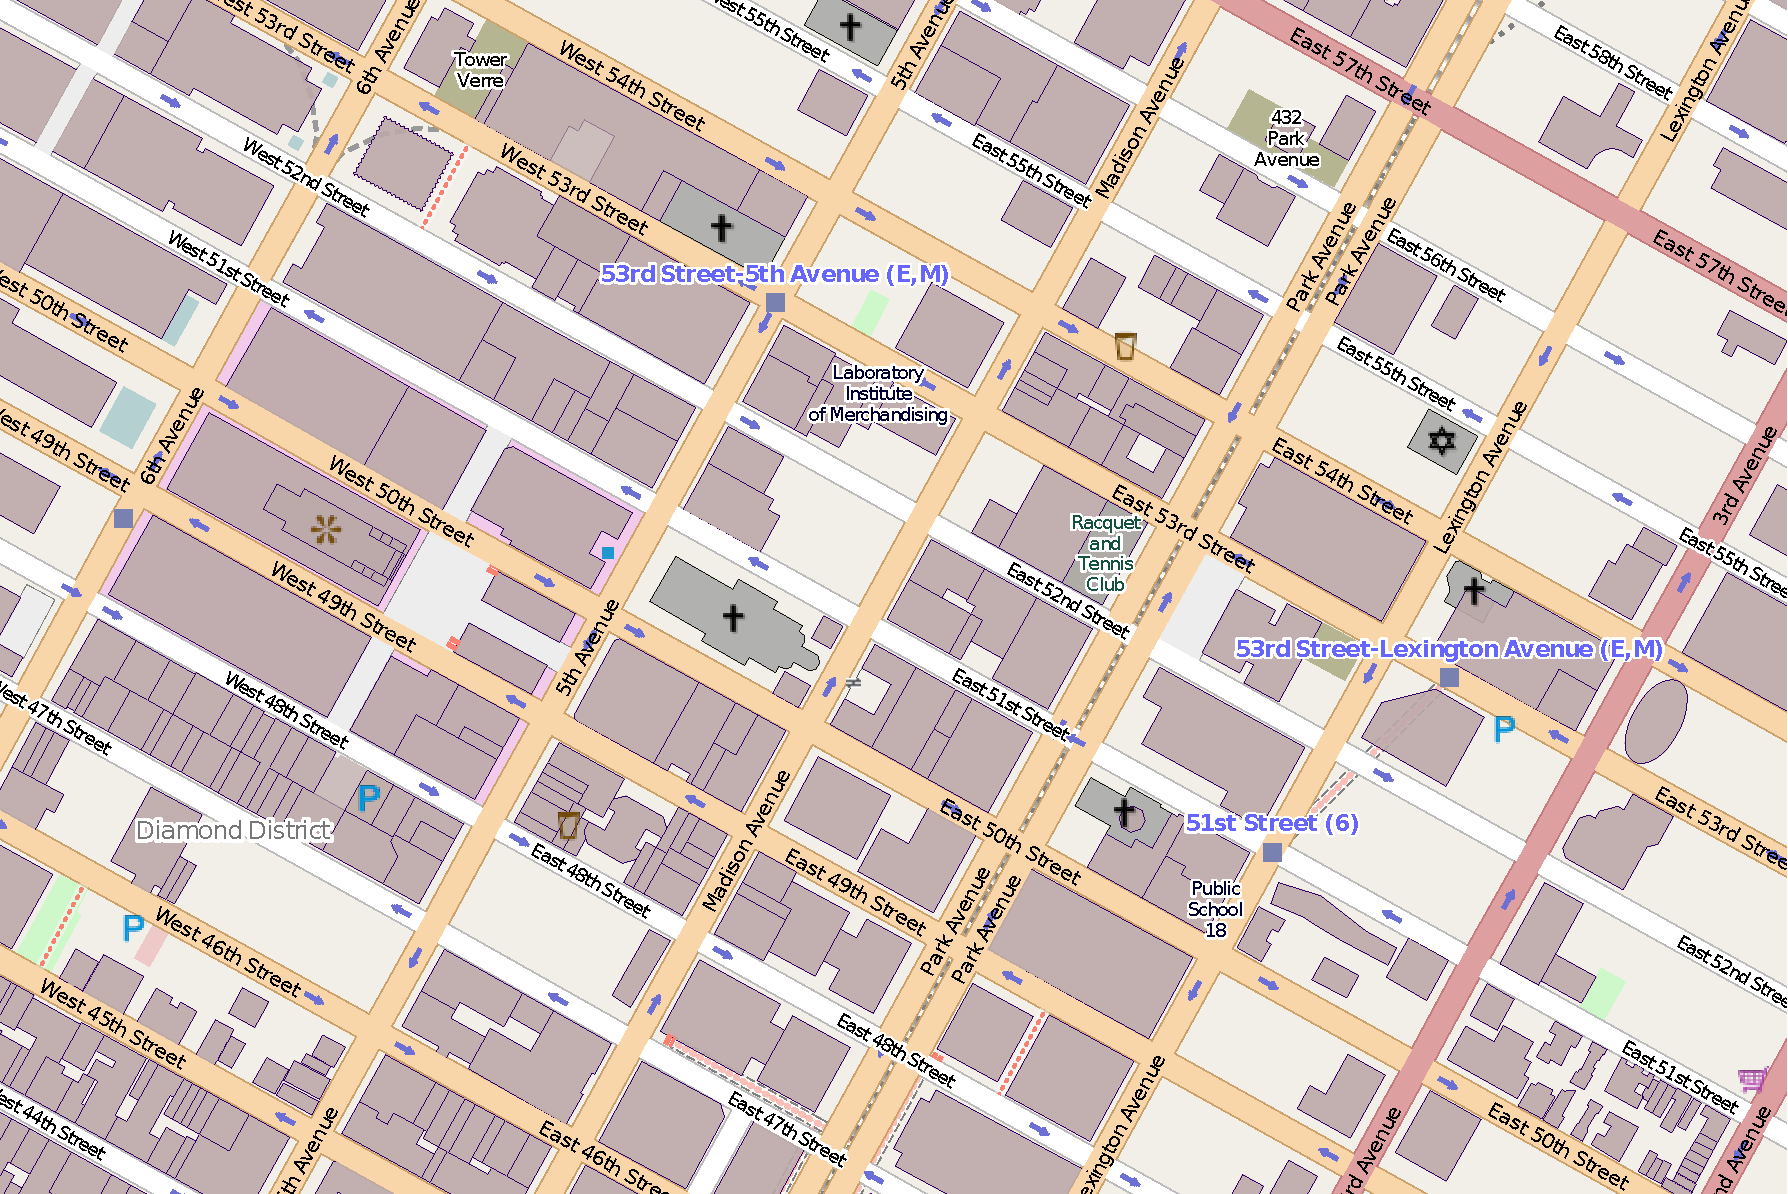
\includegraphics[width=0.94\linewidth]{images/manhattan}
\end{center}
\caption{A generated road system for Manhattan and a real map of Manhattan for comparison \cite{parish01}}
\label{fig:manhattan}
\end{figure}

\newpage
\noindent
An alternative approach is presented by Sun et al.\ in \cite{sun02}. In their paper \emph{"Template-Based Generation of Road Networks
for Virtual City Modeling"} they propose a method to generate traffic networks based on templates and a rule-based generation system. Their system uses input data in form of 2D images depicting land and water boundaries, population distribution or elevation in order to derive a suitable template which is used to create street maps of various patterns.\\

\noindent
Sun et al.\ present various road patterns which can be generated using the associated template. Each template consists of a set of rules, which define the overall road structure, and a set of parameters, which can be used to manipulate the generation system.\\

\begin{figure}[H]
\begin{center}
\includegraphics[width=0.84\linewidth]{images/roadpatterns}
\end{center}
\caption{Different road patterns presented in \cite{sun02}}
\label{fig:roadpatterns}
\end{figure}

\noindent
For each of the road patterns depicted in figure \ref{fig:roadpatterns} a corresponding template is designed. The \emph{population-based} template bases on the assumption that roads in an area with a higher population are denser in order to mitigate the traffic flow, whereas streets in less populated regions are sparse. Sun et al.\ use density points which are extracted from the population density map as input site for a Voronoi diagram. The resulting edges of this diagram represent the created road network. The \emph{raster} and \emph{radial} template just serve as a mechanism for growing patterns. The algorithm presented in \cite{sun02} starts generating vertices iteratively until it reaches the map's bounding box. The generated vertices are linked in pairs afterwards in order to create a road network. The \emph{mixed} template represents a composition of one or more of the three other patterns.\\

\noindent
The templates which are derived from various input maps represent only the envisioned (highway) road pattern. After the coarse road pattern has been generated a validity control is executed which detects roads crossing illegal areas in the map and either tries to bypass the illegal areas or discards the concerned road segment. In the next steps possible dead ends are interconnected and the road's shape is modified based on the assumption that roads are often curved naturally in order to avoide large gradients or obstructions due to different altitudes for example. The final step is the creation of minor roads covering local transport areas. This is done by extracting the regions which are seperated by the highways -- representing those local transport areas -- in the first place and generating the streets within this extracted regions afterwards. Sun et al.\ use the raster pattern for the generation of streets. After this final generation step the generated road map contains both highways interconnecting the local transport areas and minor streets covering these transport regions. An example for a generated road map is shown in figure \ref{fig:roadmap}. \\

\begin{figure}[H]
\begin{center}
\includegraphics[width=0.62\linewidth]{images/roadmap}
\end{center}
\caption{A generated road map with highways and streets \cite{sun02}}
\label{fig:roadmap}
\end{figure}